\documentclass{article}
\usepackage{graphicx} % Required for inserting images
\usepackage{hyperref}

\title{Assignment 4}
\author{Pradyumnan R}
\date{June 2023}

\begin{document}

\maketitle

\section{AE22B009}

\textbf{Name :} Pradyumnan R

\bigskip

\noindent\textbf{Github User ID :} 135097712

\begin{equation}\label{1D}
    \frac{\partial u}{\partial t} + u\frac{\partial u}{\partial x} = \nu \frac{\partial^2 u}{\partial x^2}
\end{equation}

\bigskip

\begin{flushleft}
    The above equation is called the \textit{Burgers-Bateman equation} \cite{Musha_1978} and is a convection-diffusion partial differential equation with a lot of application in applied mathematics. For instance, in aerospace engineering, it's used to analyse fluid mechanics and gas dynamics models. The equation \ref{1D} represents the $1D$ version of the Burgers-Bateman equation. 

\bigskip

    Here,

    \bigskip
    
    $u$ is the speed of the fluid at a specific point $x$ at a specific instant $t$,

    \medskip

    $\nu$ is the viscosity of the fluid

    \bigskip

    If we say that the fluid is inviscid $(\nu=0)$, we get the inviscid Burgers-Bateman equation given by,

    \begin{equation}\label{inviscid}
        \frac{\partial u}{\partial t} + u \frac{\partial^2 u}{\partial x^2} = 0
    \end{equation}

    \bigskip

    When the diffusion equation is solved by applying the \textit{Cole-Hopf transformation} \cite{evans2022partial}, and then inverting it, we get the solution to the viscous Burger-Bateman equation given by,

    \begin{equation}
        u(x,t) = -2\nu \frac{\partial}{\partial x} ln \left\{ (4\pi\nu t)^{-1/2} \int_{-\infty}^{-\infty}exp \left[ -\frac{(x-x')^2}{4\nu t} - \frac{1}{2\nu} \int_{0}^{\infty} f (x'')dx'' \right] dx' \right\}
    \end{equation}

    \bigskip

    where,

    \bigskip

    $f(x) = u(x,0)$, that is $f(x)$ represents the initial conditions.

    \bigskip

    The figure \ref{Evolution} will illustrate the history of the Burgers-Bateman equation.

    \bigskip

    \begin{figure}[h]
        \centering
            \begin{frame}{Frame Title}
                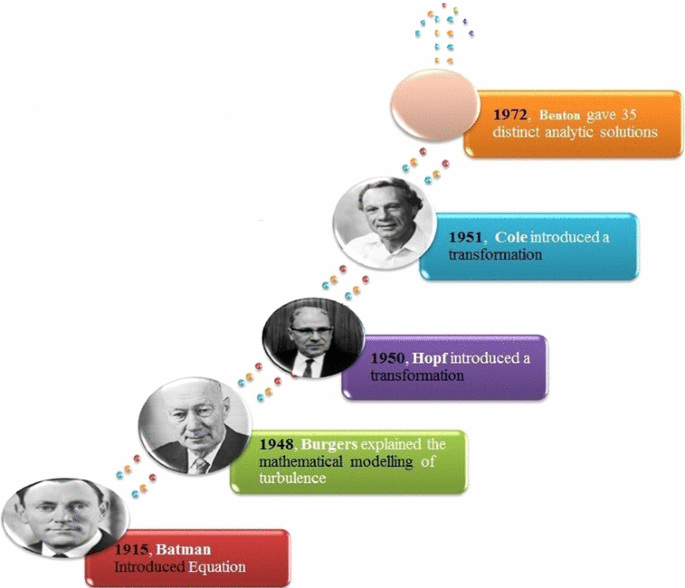
\includegraphics[scale=0.5]{Image.png}
            \end{frame}
        \caption{Evolution of the Burgers-Bateman Equation}
        \label{Evolution}
    \end{figure}
    
    
\end{flushleft}

\bibliography{bibliography.bib}
\bibliographystyle{plain}

\end{document}
